\documentclass{article}
\usepackage{graphicx} 
\usepackage{kotex}
\usepackage{listings}


\title{프로그래밍 언어 HW3 제출}
\author{C335186 서장훈}
\date{May 3, 2025}

\begin{document}

\maketitle

\section{YACC 동작 방식}


YACC는 컴파일러의 구문 분석기를 자동으로 만들어주는 도구이다. 여기서 구문 분석기란 파서라고도 불리며, 보통 Lex라는 어휘분석기 생성 도구와 함께 쓰인다. 이들은 사용자가 직접 정의한 문법을 기반으로 분석하고 작동된다. \\
\\
어휘 분석기는 보통 .l 확장자 파일로 작성된다. 코드에서 \texttt{IDENTIFIER, CONSTANT} 같은 토큰 단위의 조각들을 구분하는 역할을 한다. \\
그럼 이제 .l 파일에 정의된 패턴에 따라 토큰을 나누는 어휘 분석기를 생성해줘야 하는데, 그게 바로 lex이다. 작성된 .l 파일은 lex를 통해 처리된다. 그리고 이것을 컴파일하면 lex.yy.c 라는 c 파일이 생성된다. 이 파일은 어휘 분석기 역할을 수핼하고 코드의 각 단어를 읽고 토큰을 판별한 뒤 YACC로 전달한다. YACC는 이 토큰들의 순서와 조합을 미리 정의한 문법 규칙에 맞는지 확인하고, 맞다면 해당 규칙에 연결된 동작 코드도 실행한다. \\
\\
정리하자면 YACC는 사용자가 정의한 문법 규칙으로 코드를 분석하고, 동작을 수행하는 구문 분석기를 생성해주는 도구인 것이다. 일반적으로 lex와 함께 사용되며 lex는 입력을 토큰 단위로 분석하는 어휘 분석기를 생성한다. YACC는 그 토큰들을 이용하여 문법 구조를 판단하고 원하는 기능을 수행할 수 있도록 도와주는 것이다. \\
\\
이번 과제로 C 언어 코드에서 등장하는 함수 정의 및 호출, 연산자 사용, 변수 선언 등 특정 상황의 횟수를 카운팅하는 프로그램을 구현했다. 
YACC의 내부 동작은 크게 문법을 인식하고 의미값을 전달하고 동작을 수행한다는 두 흐름으로 나뉜다. 먼저 lex에 의해 입력된 토큰이 YACC에 전달되면 YACC는 현재 상태에서의 적용 가능한 문법 규칙을 판단하고 이를 reduce 한다. 여기서 reduce란 지금까지 읽은 단어들이 어떤 문법 구조 하나를 만족했으니, 그걸 하나의 비단말 기호로 줄이는 과정이다. 다시 말해 하위 구성 요소들을 하나의 더 큰 문법 단위로 인식하고, 비단말 기호로 치환하는 과정이라 볼 수 있겠다. 다시 본론으로 돌아가자면 이렇게 reduce된 문법 구조에 연결된 c 코드블럭이 실행되고 이곳에 카운팅 코드를 넣어두었다. \\
\\
예를 들어 연산자 같은 경우에는  \texttt{additive expression, multiplicative expression, assignment expression} 등 여러 규칙에서 등장할 수 있기 때문에 각각의 규칙 안에서 연산자가 등장할 때마다 \texttt{ary[1]++;} 를 실행하는 방식으로 처리하였다.


\section{hw3.l}

\subsection{hw3.l 코드}
\begin{lstlisting}
%{
#include <stdio.h>
#include "y.tab.h"
%}

D   [0-9]
L   [a-zA-Z_]
H   [a-fA-F0-9]
E   [Ee][+-]?{D}+
FS  (f|F|l|L)
IS  (u|U|l|L)*

%%
"/*"([^*]|(\*+[^/]))*"*/" {}
"//".* {}

"define" {return DEFINE;}
"include" {return INCLUDE;}
"int" {return INT;}
"char" {return CHAR;}
"void" {return VOID;}
"for" {return FOR;}
"while" {return WHILE;}
"do" {return DO;}
"if" {return IF;}
"switch" {return SWITCH;}
"return" {return RETURN;}
"auto" {return AUTO;}
"break" {return BREAK;}
"case" {return CASE;}
"const" {return CONST;}
"continue" {return CONTINUE;}
"default" {return DEFAULT;}
"double" {return DOUBLE;}
"enum" {return ENUM;}
"extern" {return EXTERN;}
"float" {return FLOAT;}
"goto" {return GOTO;}
"long" {return LONG;}
"register" {return REGISTER;}
"short" {return SHORT;}
"signed" {return SIGNED;}
"sizeof" {return SIZEOF;}
"static" {return STATIC;}
"struct" {return STRUCT;}
"typedef" {return TYPEDEF;}
"union" {return UNION;}
"unsigned" {return UNSIGNED;}
"volatile" {return VOLATILE;}

{L}+"."h {return HEADER;}
{L}({L}|{D})* {return IDENTIFIER;}
{D}+ {return CONSTANT;}
0[xX]{H}+{IS}? {return CONSTANT;}
0{D}+{IS}? {return CONSTANT;}
{D}+{IS}? {return CONSTANT;}
L?'(\\.|[^\\'])+' {return CONSTANT;}
{D}+{E}{FS}? {return CONSTANT;}
{D}*"."{D}+({E})?{FS}? {return CONSTANT;}
{D}+"."{D}*({E})?{FS}? {return CONSTANT;}

L?"(\\.|[^\\"])*" {return STRING_LITERAL;}

"..." {return ELLIPSIS;}
">>=" {return RIGHT_ASSIGN;}
"<<=" {return LEFT_ASSIGN;}
"+=" {return ADD_ASSIGN;}
"-=" {return SUB_ASSIGN;}
"*=" {return MUL_ASSIGN;}
"/=" {return DIV_ASSIGN;}
"%=" {return MOD_ASSIGN;}
"&=" {return AND_ASSIGN;}
"^=" {return XOR_ASSIGN;}
"|=" {return OR_ASSIGN;}
">>" {return RIGHT_OP;}
"<<" {return LEFT_OP;}
"++" {return INC_OP;}
"--" {return DEC_OP;}
"->" {return PTR_OP;}
"&&" {return AND_OP;}
"||" {return OR_OP;}
"<=" {return LE_OP;}
">=" {return GE_OP;}
"==" {return EQ_OP;}
"!=" {return NE_OP;}
";" {return ';';}
("{"|"<%") {return '{';}
("}"|"%>") {return '}';}
"," {return ',';}
":" {return ':';}
"=" {return '=';}
"(" {return '(';}
")" {return ')';}
("["|"<:") {return '[';}
("]"|":>") {return ']';}
"." {return '.';}
"&" {return '&';}
"!" {return '!';}
"~" {return '~';}
"-" {return '-';}
"+" {return '+';}
"*" {return '*';}
"/" {return '/';}
"%" {return '%';}
"<" {return '<';}
">" {return '>';}
"^" {return '^';}
"|" {return '|';}
"?" {return '?';}
"#" {return '#';}

[ \t\v\n\f] {}
. {}

%%

int yywrap(){
  return 1;
}
\end{lstlisting}

\subsection{2.2 hw3.l 코드 분석}

\begin{itemize}

  \item \textbf{규칙절 분석}
  \begin{itemize}
    \item \textbf{주석}: \texttt{//}, \texttt{/* */} 형식의 주석을 감지하고 무시한다. (과제 K-10 조건)
    \item \textbf{전처리 지시어}: \texttt{\#define}, \texttt{\#include}를 토큰으로 반환하며, \texttt{HEADER}는 \texttt{stdio.h}처럼 .h로 끝나는 경우에 인식된다. (K-3, K-4 조건) 추가로 \texttt{\#} 과 \texttt{DEFINE, INCLUDE} 를 정의했다.
    \item \textbf{자료형 및 키워드 인식}: \texttt{int}, \texttt{char}, \texttt{float} 등의 ANSI C 자료형 키워드를 인식하고 해당 토큰을 반환한다.
    \item \textbf{식별자}: 영문자 또는 밑줄로 시작하며, 영문자나 숫자를 포함할 수 있는 식별자는 \texttt{IDENTIFIER}로 반환된다.
    \item \textbf{상수}: 정수(10진수, 8진수, 16진수), 문자, 실수(지수형 포함) 등 다양한 리터럴을 \texttt{CONSTANT}로 처리한다. (K-6 조건)
    \item \textbf{문자열 상수}: \texttt{"..."}로 감싸인 문자열은 \texttt{STRING\_LITERAL}로 반환된다.
    \item \textbf{연산자 및 대입 연산자}: 복합 대입 연산자(+=, -= 등), 논리 연산자(\&\&, ||), 비교 연산자(==, != 등) 등을 토큰으로 반환한다.
    \item \textbf{기호 문자}: 괄호, 세미콜론, 쉼표 등 다양한 구문 구성 요소들도 각각의 문자 그대로 반환되며 yacc 문법에서 사용된다.
    \item \textbf{공백 및 기타}: 공백 문자는 무시되며, 알 수 없는 문자는 아무 동작 없이 무시된다.
  \end{itemize}

  \item \textbf{사용자 정의 함수}
  \begin{itemize}
    \item \texttt{yywrap()}: 입력의 끝을 처리하기 위한 표준 함수로, 1을 반환하여 입력이 끝난 것을 알린다.
  \end{itemize}
\end{itemize}

\newpage 

\section{hw3.y}

\subsection{hw3.y 코드}
\begin{lstlisting}

%{
#include <stdio.h>
int ary[9] = {0,0,0,0,0,0,0,0,0};

int cnt_v = 0;
int type(int t);
%}
%union { int type_id; }
%type <type_id> type_specifier declaration init_declarator_list
%type <type_id> parameter_declaration declaration_specifiers 
%token DEFINE INCLUDE HEADER
%token <type> INT CHAR
%token VOID FOR WHILE DO IF SWITCH RETURN
%token AUTO BREAK CASE CONST CONTINUE DEFAULT DOUBLE ENUM EXTERN
%token FLOAT GOTO LONG REGISTER SHORT SIGNED SIZEOF STATIC STRUCT
%token TYPEDEF UNION UNSIGNED VOLATILE

%token IDENTIFIER CONSTANT STRING_LITERAL

%token ELLIPSIS
%token RIGHT_ASSIGN LEFT_ASSIGN ADD_ASSIGN SUB_ASSIGN
%token MUL_ASSIGN DIV_ASSIGN MOD_ASSIGN AND_ASSIGN XOR_ASSIGN OR_ASSIGN TYPE_NAME
%token RIGHT_OP LEFT_OP INC_OP DEC_OP PTR_OP
%token AND_OP OR_OP LE_OP GE_OP EQ_OP NE_OP

%start translation_unit
%%

primary_expression
	: IDENTIFIER
	| CONSTANT
	| STRING_LITERAL
	| '(' expression ')'
	;

postfix_expression
	: primary_expression
	| postfix_expression '[' expression ']'
	| postfix_expression '(' ')' {ary[0]++;}
	| postfix_expression '(' argument_expression_list ')'  {ary[0]++;}
	| postfix_expression '.' IDENTIFIER {ary[1]++;}
	| postfix_expression PTR_OP IDENTIFIER {ary[1]++;}
	| postfix_expression INC_OP {ary[1]++;}
	| postfix_expression DEC_OP {ary[1]++;}
	;

argument_expression_list
	: assignment_expression
	| argument_expression_list ',' assignment_expression
	;

unary_expression
	: postfix_expression
	| INC_OP unary_expression {ary[1]++;}
	| DEC_OP unary_expression {ary[1]++;}
	| unary_operator cast_expression 
	| SIZEOF unary_expression
	| SIZEOF '(' type_name ')'
	;

unary_operator
	: '&'
	| '*'
	| '+'
	| '-'
	| '~'
	| '!'
	;

cast_expression
	: unary_expression
	| '(' type_name ')' cast_expression {ary[1]++;} 
	;

multiplicative_expression
	: cast_expression
	| multiplicative_expression '*' cast_expression {ary[1]++;}
	| multiplicative_expression '/' cast_expression {ary[1]++;}
	| multiplicative_expression '%' cast_expression {ary[1]++;}
	;

additive_expression
	: multiplicative_expression
	| additive_expression '+' multiplicative_expression {ary[1]++;}
	| additive_expression '-' multiplicative_expression {ary[1]++;}
	;

shift_expression
	: additive_expression
	| shift_expression LEFT_OP additive_expression {ary[1]++;}
	| shift_expression RIGHT_OP additive_expression {ary[1]++;}
	;

relational_expression
	: shift_expression
	| relational_expression '<' shift_expression {ary[1]++;}
	| relational_expression '>' shift_expression {ary[1]++;}
	| relational_expression LE_OP shift_expression {ary[1]++;}
	| relational_expression GE_OP shift_expression {ary[1]++;}
	;

equality_expression
	: relational_expression
	| equality_expression EQ_OP relational_expression {ary[1]++;}
	| equality_expression NE_OP relational_expression {ary[1]++;}
	;

and_expression
	: equality_expression
	| and_expression '&' equality_expression {ary[1]++;}
	;

exclusive_or_expression
	: and_expression
	| exclusive_or_expression '^' and_expression {ary[1]++;}
	;

inclusive_or_expression
	: exclusive_or_expression
	| inclusive_or_expression '|' exclusive_or_expression {ary[1]++;}
	;

logical_and_expression
	: inclusive_or_expression
	| logical_and_expression AND_OP inclusive_or_expression {ary[1]++;}
	;

logical_or_expression
	: logical_and_expression
	| logical_or_expression OR_OP logical_and_expression {ary[1]++;}
	;

conditional_expression
	: logical_or_expression
	| logical_or_expression '?' expression ':' conditional_expression
	;

assignment_expression
	: conditional_expression
	| unary_expression assignment_operator assignment_expression
	;

assignment_operator
	: '='  {ary[1]++;}
	| MUL_ASSIGN {ary[1]++;}
	| DIV_ASSIGN {ary[1]++;}
	| MOD_ASSIGN {ary[1]++;}
	| ADD_ASSIGN {ary[1]++;}
	| SUB_ASSIGN {ary[1]++;}
	| LEFT_ASSIGN {ary[1]++;}
	| RIGHT_ASSIGN {ary[1]++;}
	| AND_ASSIGN {ary[1]++;}
	| XOR_ASSIGN {ary[1]++;}
	| OR_ASSIGN {ary[1]++;}
	;

expression
	: assignment_expression
	| expression ',' assignment_expression
	;

constant_expression
	: conditional_expression
	;

declaration
	: declaration_specifiers ';'{cnt_v = 0; $$ = $1;}
	| declaration_specifiers init_declarator_list ';' {
		for (int i = 0; i < cnt_v; i++) type($1);
		$$ = $1;
	}
	;

declaration_specifiers
	: storage_class_specifier {$$ = 0;}
	| storage_class_specifier declaration_specifiers  {$$ = 0;}
	| type_specifier  {$$ = $1;}
	| type_specifier declaration_specifiers {$$ = $1;}
	| type_qualifier {$$ = 0;}
	| type_qualifier declaration_specifiers {$$ = 0;}
	;

init_declarator_list
	: init_declarator {cnt_v = 1;}
	| init_declarator_list ',' init_declarator {cnt_v++;}
	;

init_declarator
	: declarator
	| declarator '=' initializer {ary[1]++;}
	;

storage_class_specifier
	: TYPEDEF
	| EXTERN
	| STATIC
	| AUTO
	| REGISTER
	;

type_specifier
	: VOID {$$ = 0;}
	| CHAR {$$ = 3;}
	| SHORT {$$ = 0;}
	| INT {$$ = 2;}
	| LONG {$$ = 0;}
	| FLOAT {$$ = 0;}
	| DOUBLE {$$ = 0;}
	| SIGNED {$$ = 0;}
	| UNSIGNED {$$ = 0;}
	| struct_or_union_specifier {$$ = 0;}
	| enum_specifier {$$ = 0;}
	| TYPE_NAME {$$ = 0;}
	;

struct_or_union_specifier
	: struct_or_union IDENTIFIER '{' struct_declaration_list '}'
	| struct_or_union '{' struct_declaration_list '}'
	| struct_or_union IDENTIFIER
	;

struct_or_union
	: STRUCT
	| UNION
	;

struct_declaration_list
	: struct_declaration
	| struct_declaration_list struct_declaration
	;

struct_declaration
	: specifier_qualifier_list struct_declarator_list ';'
	;

specifier_qualifier_list
	: type_specifier specifier_qualifier_list
	| type_specifier
	| type_qualifier specifier_qualifier_list
	| type_qualifier
	;

struct_declarator_list
	: struct_declarator
	| struct_declarator_list ',' struct_declarator
	;

struct_declarator
	: declarator
	| ':' constant_expression
	| declarator ':' constant_expression
	;

enum_specifier
	: ENUM '{' enumerator_list '}'
	| ENUM IDENTIFIER '{' enumerator_list '}'
	| ENUM IDENTIFIER
	;

enumerator_list
	: enumerator
	| enumerator_list ',' enumerator
	;

enumerator
	: IDENTIFIER
	| IDENTIFIER '=' constant_expression  {ary[1]++;}
	;

type_qualifier
	: CONST
	| VOLATILE
	;

declarator
	: pointer direct_declarator {ary[4]++;}
	| direct_declarator
	;

direct_declarator
	: IDENTIFIER
	| '(' declarator ')'
	| direct_declarator '[' constant_expression ']' {ary[5]++;}
	| direct_declarator '[' ']' {ary[5]++;}
	| direct_declarator '(' parameter_type_list ')'
	| direct_declarator '(' identifier_list ')'
	| direct_declarator '(' ')'
	;

pointer
	: '*'
	| '*' type_qualifier_list
	| '*' pointer
	| '*' type_qualifier_list pointer
	;

type_qualifier_list
	: type_qualifier
	| type_qualifier_list type_qualifier
	;


parameter_type_list
	: parameter_list
	| parameter_list ',' ELLIPSIS
	;

parameter_list
	: parameter_declaration
	| parameter_list ',' parameter_declaration
	;

parameter_declaration
	: declaration_specifiers declarator {type($1);}
	| declaration_specifiers abstract_declarator {type($1);}
	| declaration_specifiers
	;

identifier_list
	: IDENTIFIER
	| identifier_list ',' IDENTIFIER
	;

type_name
	: specifier_qualifier_list
	| specifier_qualifier_list abstract_declarator
	;

abstract_declarator
	: pointer  {ary[4]++;}
	| direct_abstract_declarator
	| pointer direct_abstract_declarator {ary[4]++;}
	;

direct_abstract_declarator
	: '(' abstract_declarator ')'
	| '[' ']'
	| '[' constant_expression ']'
	| direct_abstract_declarator '[' ']'
	| direct_abstract_declarator '[' constant_expression ']'
	| '(' ')'
	| '(' parameter_type_list ')'
	| direct_abstract_declarator '(' ')'
	| direct_abstract_declarator '(' parameter_type_list ')'
	;

initializer
	: assignment_expression
	| '{' initializer_list '}'
	| '{' initializer_list ',' '}'
	;

initializer_list
	: initializer
	| initializer_list ',' initializer
	;

statement
	: labeled_statement
	| compound_statement
	| expression_statement
	| selection_statement
	| iteration_statement
	| jump_statement
	;

labeled_statement
	: IDENTIFIER ':' statement
	| CASE constant_expression ':' statement
	| DEFAULT ':' statement
	;

compound_statement
	: '{' '}'
	| '{' hw3_statement_list '}'
	;

declaration_list
	: declaration
	| declaration_list declaration
	;

hw3_statement_list
	: hw3_statement
	| hw3_statement_list hw3_statement
	;

hw3_statement
	: declaration
	| statement
	;

expression_statement
	: ';'
	| expression ';'
	;

selection_statement
	: IF '(' expression ')' statement {ary[6]++;}
	| SWITCH '(' expression ')' statement {ary[6]++;}
	;

iteration_statement
	: WHILE '(' expression ')' statement {ary[7]++;}
	| DO statement WHILE '(' expression ')' ';' {ary[7]++;}
	| FOR '(' expression_statement expression_statement ')' statement {ary[7]++;}
	| FOR '(' expression_statement expression_statement expression ')' statement {ary[7]++;}
	;

jump_statement
	: GOTO IDENTIFIER ';'
	| CONTINUE ';'
	| BREAK ';'
	| RETURN ';'  {ary[8]++;}
	| RETURN expression ';' {ary[8]++;}
	;

translation_unit
	: external_declaration
	| translation_unit external_declaration
	;

external_declaration
	: function_definition
	| declaration
	| include_process
	| define_process
	;

function_definition
	: declaration_specifiers declarator declaration_list compound_statement  {ary[0]++; type($1);}
	| declaration_specifiers declarator compound_statement {ary[0]++;}
	| declarator declaration_list compound_statement {ary[0]++;}
	| declarator compound_statement {ary[0]++;}
	;

include_process
	: '#' INCLUDE '<' HEADER '>'
	| '#' INCLUDE '"' HEADER '"'
	;

define_process
	: '#' DEFINE IDENTIFIER CONSTANT
	;


%%

int main(void)
{
	yyparse();
	printf("function = %d\n", ary[0]);
	printf("operator = %d\n", ary[1]);
	printf("int = %d\n", ary[2]);
	printf("char = %d\n", ary[3]);
	printf("pointer = %d\n", ary[4]);
	printf("array = %d\n", ary[5]);
	printf("selection = %d\n", ary[6]);
	printf("loop = %d\n", ary[7]);
	printf("return = %d\n", ary[8]);
	return 0;
}

void yyerror(const char *str)
{
	fprintf(stderr, "error: %s\n", str);
}


int type(int t) {
    if (t == 2 || t == 3) {
        ary[t]++;
    }
    return t;
}
\end{lstlisting}

코드의 전체 구성을 이러하다.


\section{hw3.y 코드 분석}

각각의 블럭은 YACC의 동작 중 특정 문법 규칙이 reduce 될 때 실행되는 액션으로 구성되어 있다.
A~I 조건을 충족하기 위해 어떻게 작성되었는지를 중심으로 분석을 할 예정이다. 



\subsection{함수 호출 카운팅}

\texttt{hw3.y} 파일 내에서 함수 호출은 다음과 같은 YACC 문법으로 정의되어 있으며, 호출이 감지될 때마다 \texttt{ary[0]}의 값이 1씩 증가하게 된다. 이는 과제 명세 조건 \textbf{A. Function}에 해당한다.

\begin{lstlisting}
postfix_expression
    : primary_expression
    | postfix_expression '[' expression ']'
    | postfix_expression '(' ')' { ary[0]++; }
    | postfix_expression '(' argument_expression_list ')' { ary[0]++; }
    ...
\end{lstlisting}

위 문법에서 함수 호출을 처리하는 부분은 두 가지 production이다.

\begin{itemize}
  \item \texttt{postfix\_expression '(' ')'} : 인자가 없는 함수 호출을 나타낸다. 예를 들어 \texttt{foo();}와 같이 사용된 경우이다. 이 경우 \texttt{ary[0]++}가 수행된다.
  \item \texttt{postfix\_expression '(' argument\_expression\_list ')'} : 인자를 포함한 함수 호출을 나타낸다. 예를 들어 \texttt{foo(1, 2);}와 같은 표현이 이 문법에 매칭되며, 마찬가지로 \texttt{ary[0]++}가 수행된다.
\end{itemize}

이러한 카운팅 로직은 다음과 같은 방식으로 동작한다.


\begin{enumerate}
  \item \textbf{\texttt{postfix\_expression}이 \texttt{IDENTIFIER}로 시작} \\
  기본적으로 함수명은 \texttt{IDENTIFIER} 토큰으로 분석된다. 이 토큰은 Lex에서 정의된 정규식 \texttt{{L}({L}|{D})*}에 따라 인식된다.

  \item \textbf{괄호 \texttt{( )} 또는 \texttt{( argument )}가 뒤따라오는 경우} \\
  이는 해당 \texttt{IDENTIFIER}가 단순한 변수명이 아니라, 실제로 함수 호출이라는 것을 의미한다. 이 규칙은 \texttt{postfix\_expression}에서 처리된다.

  \item \textbf{해당 production에 도달하면 \texttt{ary[0]++} 수행} \\
  YACC는 \texttt{postfix\_expression '(' ')'} 또는 \texttt{postfix\_expression '(' argument\_expression\_list ')'}의 패턴을 인식할 때마다, 명시적으로 \texttt{ary[0]++}를 실행하여 함수 호출 횟수를 카운팅한다.
\end{enumerate}


\paragraph{예시 분석}
다음과 같은 코드가 있다고 하자.

\begin{lstlisting}[language=C]
int main() {
    printf("programing language HW3\n");
    add(1, 2);
    get_value();
}
\end{lstlisting}

Lex 단계에서 다음과 같은 토큰이 생성된다:

\begin{itemize}
  \item \texttt{printf} $\rightarrow$ \texttt{IDENTIFIER}
  \item \texttt{(} $\rightarrow$ '('
  \item \texttt{"programing language HW3\textbackslash n"} $\rightarrow$ \texttt{STRING\_LITERAL}
  \item \texttt{)} $\rightarrow$ ')'
  \item \texttt{;} $\rightarrow$ ';'
\end{itemize}

YACC는 위 토큰들을 조합하여 \texttt{postfix\_expression '(' argument\_expression\_list ')'} production을 인식하게 되며, 이로 인해 \texttt{ary[0]}이 \texttt{1} 증가한다. 이후 \texttt{add(1, 2)}와 \texttt{get\_value()}도 동일하게 인식되며, 호출마다 카운트가 증가하여 최종적으로 \texttt{ary[0] = 3}이 된다.


\paragraph{정리}
\begin{itemize}
  \item 호출 감지는 \texttt{postfix\_expression} 문법 내 괄호 패턴으로 수행된다.
  \item 호출 카운트는 \texttt{ary[0]++}로 처리된다.
  \item 정의는 \texttt{function\_definition}에서 별도로 카운트된다.
  \item 선언만 있는 함수는 카운트 대상이 아니다.
\end{itemize}

이처럼 함수 호출은 호출 방식(인자 유무)과 관계없이 정확히 하나씩 카운트되며, 선언과 정의, 호출 간의 처리를 분리함으로써 요구된 명세에 따라 정확한 기능 분석이 가능하게 되어 있다.

\subsection{연산자(operator) 분석}

B에서 \textbf{모든 이항 연산자}의 사용을 카운트해야 하고 단항 연산자, 삼항 연산자, 전처리 연산자 등은 포함하지 않는다. YACC 문법 규칙 내부에서 연산자가 등장할 때마다 \texttt{ary[1]++}을 호출하여 카운트한다.

\begin{itemize}
  \item \textbf{증감 연산자}
  \begin{lstlisting}
postfix_expression INC_OP { ary[1]++; }
postfix_expression DEC_OP { ary[1]++; }
unary_expression INC_OP unary_expression { ary[1]++; }
unary_expression DEC_OP unary_expression { ary[1]++; }
  \end{lstlisting}
  \begin{itemize}
    \item 후위 및 전위의 증감 연산자를 모두 이항 연산자처럼 취급하여 카운트한다.
  \end{itemize}

  \item \textbf{산술 연산자}
  \begin{lstlisting}
multiplicative_expression '*' cast_expression { ary[1]++; }
multiplicative_expression '/' cast_expression { ary[1]++; }
multiplicative_expression '%' cast_expression { ary[1]++; }
additive_expression '+' multiplicative_expression { ary[1]++; }
additive_expression '-' multiplicative_expression { ary[1]++; }
  \end{lstlisting}
  \begin{itemize}
    \item 일반적인 산술 이항 연산자 모두 조건 B에 해당한다.
  \end{itemize}

  \item \textbf{비트 이동 연산자}
  \begin{lstlisting}
shift_expression LEFT_OP additive_expression { ary[1]++; }
shift_expression RIGHT_OP additive_expression { ary[1]++; }
  \end{lstlisting}
  \begin{itemize}
    \item 비트 시프트 연산자도 이항 연산자이므로 포함한다.
  \end{itemize}

  \item \textbf{비교 연산자}
  \begin{lstlisting}
relational_expression '<' shift_expression { ary[1]++; }
relational_expression '>' shift_expression { ary[1]++; }
relational_expression LE_OP shift_expression { ary[1]++; }
relational_expression GE_OP shift_expression { ary[1]++; }
  \end{lstlisting}
  \begin{itemize}
    \item 관계 연산자 또한 조건에 포함되므로 포함한다.
  \end{itemize}

  \item \textbf{등가 연산자}
  \begin{lstlisting}
equality_expression EQ_OP relational_expression { ary[1]++; }
equality_expression NE_OP relational_expression { ary[1]++; }
  \end{lstlisting}
  \begin{itemize}
    \item 비교 연산자도 조건은 만족하므로 포함한다.
  \end{itemize}

  \item \textbf{비트 연산자}
  \begin{lstlisting}
and_expression '&' equality_expression { ary[1]++; }
exclusive_or_expression '^' and_expression { ary[1]++; }
inclusive_or_expression '|' exclusive_or_expression { ary[1]++; }
  \end{lstlisting}
  \begin{itemize}
    \item 비트 연산도 이항 연산이므로 포함한다.
  \end{itemize}

  \item \textbf{논리 연산자}
  \begin{lstlisting}
logical_and_expression AND_OP inclusive_or_expression { ary[1]++; }
logical_or_expression OR_OP logical_and_expression { ary[1]++; }
  \end{lstlisting}
  \begin{itemize}
    \item 조건문 등에서 사용되는 논리 AND/OR 연산도 조건 B에 포함한다.
  \end{itemize}

  \item \textbf{할당 연산자}
  \begin{lstlisting}
assignment_operator '=' { ary[1]++; }
assignment_operator MUL_ASSIGN { ary[1]++; }
assignment_operator DIV_ASSIGN { ary[1]++; }
assignment_operator MOD_ASSIGN { ary[1]++; }
assignment_operator ADD_ASSIGN { ary[1]++; }
assignment_operator SUB_ASSIGN { ary[1]++; }
assignment_operator LEFT_ASSIGN { ary[1]++; }
assignment_operator RIGHT_ASSIGN { ary[1]++; }
assignment_operator AND_ASSIGN { ary[1]++; }
assignment_operator XOR_ASSIGN { ary[1]++; }
assignment_operator OR_ASSIGN { ary[1]++; }
  \end{lstlisting}
  \begin{itemize}
    \item 조건에 따라 포한한다.
  \end{itemize}

  \item \textbf{형변환 연산자}
  \begin{lstlisting}
'(' type_name ')' cast_expression { ary[1]++; }
  \end{lstlisting}
  \begin{itemize}
    \item 조건에 따라 포함한다.
  \end{itemize}

  \item \textbf{삼항 연산자 (? :)는 제외됨}
  \begin{lstlisting}
conditional_expression
  : logical_or_expression
  | logical_or_expression '?' expression ':' conditional_expression
  \end{lstlisting}
  \begin{itemize}
    \item 조건에 따라 B에서 제외한다.
  \end{itemize}
\end{itemize}

\subsubsection*{정리}

\begin{itemize}
  \item \texttt{ary[1]} 은 모든 이항 연산자와 예외적으로 포함된 단항 연산자(++, --, cast 등)의 발생 횟수를 정확히 카운트한다.
  \item \texttt{assignment\_operator}는 별도 symbol로 묶여 있어 명확한 처리 가능하다.
\end{itemize}

\subsection{int, char 카운팅 (조건 C, D)}

\texttt{int}와 \texttt{char}는 각각 조건 C, D에 해당하며, 출현 횟수를 \texttt{ary[2]}, \texttt{ary[3]}에 각각 저장한다. 

두 타입 모두 \texttt{type\_specifier} 심볼에서 분기되며, 내부적으로는 동일한 흐름으로 처리된다.

\subsubsection*{1. type\_specifier에서 카운트 분기}

\begin{lstlisting}
type_specifier
  : INT  { $$ = 2; }
  | CHAR { $$ = 3; }
\end{lstlisting}

\begin{itemize}
  \item \texttt{INT}는 \texttt{type\_id = 2}, \texttt{CHAR}는 \texttt{type\_id = 3}으로 설정된다.
  \item 실제 카운트는 여기서가 아니라, 이후 \texttt{type()} 함수에서 수행된다.
\end{itemize}

\subsubsection*{2. 선언 구문에서의 처리 (int a, char b, ...)}

\begin{lstlisting}
declaration
  : declaration_specifiers init_declarator_list ';' {
      for (int i = 0; i < cnt_v; i++) type($1);
  }
\end{lstlisting}

\begin{itemize}
  \item 변수 선언 시 \texttt{init\_declarator\_list}의 개수만큼 \texttt{cnt\_v}가 설정됨.
  \item 각 변수에 대해 \texttt{type()} 함수 호출 → int 또는 char이면 해당 ary 인덱스 증가.
\end{itemize}

\subsubsection*{3. 함수 파라미터에서의 처리}

\begin{lstlisting}
parameter_declaration
  : declaration_specifiers declarator { type($1); }
\end{lstlisting}

\begin{itemize}
  \item 파라미터 선언 구문에서도 \texttt{declaration\_specifiers}로부터 받은 \texttt{type\_id}를 \texttt{type()}에 넘겨 카운트.
\end{itemize}

\subsubsection*{4. type() 함수 구현}

\begin{lstlisting}
int type(int t) {
  if (t == 2 || t == 3) {
    ary[t]++;
  }
  return t;
}
\end{lstlisting}

\begin{itemize}
  \item \texttt{t == 2}이면 \texttt{ary[2]++} (int 카운트)
  \item \texttt{t == 3}이면 \texttt{ary[3]++} (char 카운트)
  \item 반환형으로 등장한 경우는 이 함수가 호출되지 않으므로 카운트에서 제외된다.
\end{itemize}

\subsubsection*{5. init\_declarator\_list로 변수 개수 추적}

\begin{lstlisting}
init_declarator_list
  : init_declarator { cnt_v = 1; }
  | init_declarator_list ',' init_declarator { cnt_v++; }
\end{lstlisting}

\begin{itemize}
  \item 변수 선언 항목 수를 \texttt{cnt\_v}에 누적.
  \item 이후 declaration 블록에서 \texttt{cnt\_v} 횟수만큼 \texttt{type()} 호출 → 정확한 변수 수 카운트.
\end{itemize}

\subsubsection*{6. 적용 예시별 동작 방식}

\begin{itemize}
  \item \textbf{int a;} → \texttt{type(2)} 호출 → \texttt{ary[2]++}
  \item \textbf{char c;} → \texttt{type(3)} 호출 → \texttt{ary[3]++}
  \item \textbf{int x, y, z;} → \texttt{cnt\_v = 3} → \texttt{type(2)} 3회 호출 → \texttt{ary[2] += 3}
  \item \textbf{void f(int a, char b);} → 파라미터에 대해 각각 \texttt{type(2)}, \texttt{type(3)} 호출
\end{itemize}

\subsubsection*{7. 함수 반환형의 예외 처리}

\begin{lstlisting}
function_definition
  : declaration_specifiers declarator compound_statement { ary[0]++; }
\end{lstlisting}

\begin{itemize}
  \item 함수 정의의 반환형은 \texttt{type()}을 호출하지 않거나,
  \item \texttt{declaration\_specifiers}에서 따로 카운팅 로직을 분기하지 않음.
  \item 따라서 \texttt{int f()} 또는 \texttt{char f()}는 변수 또는 파라미터로 간주되지 않아 카운트되지 않음.
\end{itemize}

\subsubsection*{8. 요약}

\begin{itemize}
  \item \texttt{INT} → \texttt{type\_id = 2}, \texttt{CHAR} → \texttt{type\_id = 3}
  \item \texttt{type()} 함수 내부에서 \texttt{ary[2]++, ary[3]++}
  \item 변수 선언은 \texttt{cnt\_v} 횟수만큼 반복 호출
  \item 파라미터 선언은 단일 호출
  \item 함수 반환형은 무시되며, 실제 count에는 포함되지 않음
\end{itemize}


\subsection{포인터 카운팅(조건 E)}

과제 명세 조건 E는 \texttt{포인터로 선언된 변수의 출현 횟수}를 카운팅하는 것을 요구한다. 이때 주의할 점은 포인터의 레벨(예: \texttt{int *}, \texttt{char **})과는 무관하게, 포인터 변수 하나당 1회로 계산된다는 것이다.


\subsubsection*{1. declarator 구문에서의 포인터 선언 인식}
\begin{lstlisting}
declarator
  : pointer direct_declarator { ary[4]++; }
  | direct_declarator
\end{lstlisting}

\begin{itemize}
  \item 포인터로 선언된 변수는 항상 \texttt{pointer direct\_declarator} 형태로 reduce 된다.
  \item 이 경우 \texttt{ary[4]}를 1 증가시킴으로써 포인터 변수 한 개가 선언되었음을 기록한다.
  \item 포인터가 2중 이상이어도 카운팅은 1회만 발생한다. (예: \texttt{int **x;}도 1회)
\end{itemize}

\subsubsection*{3. abstract\_declarator 구문에서의 포인터 선언 인식}
\begin{lstlisting}
abstract_declarator
  : pointer                   { ary[4]++; }
  | pointer direct_abstract_declarator { ary[4]++; }
\end{lstlisting}

\begin{itemize}
  \item abstract declarator는 파라미터 또는 typedef 등에서 이름 없는 타입을 지정할 때 등장.
  \item 이 경우에도 \texttt{pointer}가 등장하면 포인터로 인식하여 \texttt{ary[4]}를 증가시킨다.
\end{itemize}

\subsubsection*{4. pointer 심볼의 내부 정의}
\begin{lstlisting}
pointer
  : '*'
  | '*' type_qualifier_list
  | '*' pointer
  | '*' type_qualifier_list pointer
\end{lstlisting}

\begin{itemize}
  \item \texttt{*}는 포인터 선언의 핵심이며, qualifier 여부 또는 다중 포인터 여부에 상관없이 동일하게 처리된다.
  \item 단, 여기서 \texttt{ary[4]}를 직접 증가시키지 않고, 위 \texttt{declarator} 및 \texttt{abstract\_declarator}에서 카운팅한다.
  \item 이 구조는 중첩 포인터에서도 오직 변수 1개당 1회만 카운팅되도록 보장한다.
\end{itemize}

\subsubsection*{5. 파라미터에 포인터가 등장하는 경우}

\begin{lstlisting}
parameter_declaration
  : declaration_specifiers declarator
  | declaration_specifiers abstract_declarator
\end{lstlisting}

\begin{itemize}
  \item 포인터 파라미터도 마찬가지로 \texttt{declarator} 혹은 \texttt{abstract\_declarator}를 통해 처리되므로, 위에서 설명한 방식대로 카운트된다.
\end{itemize}

\subsubsection*{6. 적용 예시별 동작 방식}

\begin{itemize}
  \item \textbf{int *p;} → \texttt{declarator → pointer} 매칭 → \texttt{ary[4]++}
  \item \textbf{char **pp;} → 2중 포인터지만 변수는 1개 → \texttt{ary[4]++}
  \item \textbf{int *a, *b;} → \texttt{init\_declarator\_list}에서 두 개의 포인터 → \texttt{ary[4] += 2}
  \item \textbf{void f(int *ptr);} → 함수 파라미터에 포인터 → \texttt{ary[4]++}
  \item \textbf{typedef int* ptr;} → \texttt{abstract\_declarator} 경로를 통해 포인터 인식 → \texttt{ary[4]++}
\end{itemize}


\subsection{배열(array) 선언 분석}

배열 조건 F에 해당하는 부분이다.

\subsubsection*{1. 배열 문법 정의 위치}

배열은 다음과 같이 \texttt{direct\_declarator} 비단말에서 탐지된다.

\begin{lstlisting}
direct_declarator
  : IDENTIFIER
  | '(' declarator ')'
  | direct_declarator '[' constant_expression ']' { ary[5]++; }
  | direct_declarator '[' ']'                     { ary[5]++; }
  | direct_declarator '(' parameter_type_list ')'
  | direct_declarator '(' identifier_list ')'
  | direct_declarator '(' ')'
\end{lstlisting}

\texttt{'[' constant\_expression ']'} 또는 \texttt{'[' ']'} 패턴이 등장하면 배열로 간주된다. 이 경우마다 \texttt{ary[5]++} 연산이 실행되어 배열 사용을 카운트한다.

\subsubsection*{2. 동작 예시 설명}

\begin{itemize}
  \item \textbf{배열 크기 명시된 선언}:

  \begin{lstlisting}[language=C]
int arr[10];
  \end{lstlisting}
  위 코드는 YACC에서 \texttt{direct\_declarator '[' constant\_expression ']'} 패턴으로 인식되며,
  배열 선언이므로 \texttt{ary[5]++}가 실행된다. (조건 F)

  \item \textbf{크기 명시 없는 선언}:

  \begin{lstlisting}[language=C]
char buffer[] = "hi";
  \end{lstlisting}
  위 선언은 크기를 명시하지 않았지만 \texttt{[]} 패턴을 통해 배열로 인식되며, \texttt{ary[5]++}가 수행된다.

  \item \textbf{함수 파라미터로 전달된 배열}:

  \begin{lstlisting}[language=C]
void f(int param[5]);
  \end{lstlisting}
  파라미터에서 배열이 사용되어도 동일하게 \texttt{direct\_declarator} 내부에 배열 표현이 포함되며,
  역시 \texttt{ary[5]++}가 수행된다.

  \item \textbf{2차원 배열}:

  \begin{lstlisting}[language=C]
int matrix[3][3];
  \end{lstlisting}
  위 선언은 2차원 배열 표현으로, \texttt{[3][3]} 두 번 반복되지만 조건에 따라 \texttt{ary[5]++}는 한번만 발생한다.
\end{itemize}

\subsection{조건문과 반복문 구문 분석}

\begin{itemize}
  \item \textbf{조건문: if, switch}

  \begin{lstlisting}[language=C]
if (x > 0) {
  printf("no else");
}
  \end{lstlisting}
  위 코드는 \texttt{selection\_statement}에서 \texttt{IF '(' expression ')' statement}로 매칭되며, \texttt{ary[6]++}가 수행된다.

  \begin{lstlisting}[language=C]
switch (code) {
  case 1: break;
}
  \end{lstlisting}
  마찬가지로 \texttt{SWITCH '(' expression ')' statement} 패턴과 매칭되어 조건문 카운터인 \texttt{ary[6]} 값이 1 증가한한다.
  else는 조건에 따라 제외했다.

  \item \textbf{반복문: while, do while, for}

  \begin{lstlisting}[language=C]
while (i < 10) {
  i++;
}
  \end{lstlisting}
  \texttt{WHILE '(' expression ')' statement} 구문에 해당되며, \texttt{ary[7]++}가 발생한다.

  \begin{lstlisting}[language=C]
do {
  x--;
} while (x > 0);
  \end{lstlisting}
  \texttt{DO statement WHILE '(' expression ')' ';'} 형태로 reduce되며, 역시 \texttt{ary[7]++}가 된다.

  \begin{lstlisting}[language=C]
for (int i = 0; i < 5; i++) {
  printf("%d", i);
}
  \end{lstlisting}
  YACC 문법 \texttt{FOR '(' expression\_statement expression\_statement expression ')' statement}과 일치하며 반복문 카운트가 증가된다.

  \begin{lstlisting}[language=C]
for (;;) { break; }
  \end{lstlisting}
  표현식 없이 무한 루프를 구성한 for문도 유효하며, 같은 방식으로 반복문으로 인식되어 \texttt{ary[7]++} 된다.
\end{itemize}

\subsection{return, define, include, HEADER 처리}

\begin{itemize}
  \item \textbf{return 문}은 YACC의 \texttt{jump\_statement} 규칙에서 처리된다. 이렇게 과제 조건 I를 만족한다.

  \item \textbf{define 문}은 \texttt{\# DEFINE IDENTIFIER CONSTANT}의 구조로 정의되며, 마지막 항목이 상수일 때만 유효하게 처리된다. 이는 과제 조건 K-4를 만족한다.

  \item \textbf{include 문}은 \texttt{\# INCLUDE <HEADER>} 또는 \texttt{\# INCLUDE "HEADER"} 형식으로 처리되며, HEADER는 \texttt{.h} 확장자로 끝나는 문자열로 인식된다. 과제 조건 K-3과 K-4를 모두 만족한다.

  \item \textbf{HEADER 토큰}은 Lex에서 \texttt{\{L\}+"."h} 패턴으로 정의되며, \texttt{stdio.h}, \texttt{example.h}와 같은 문자열을 \texttt{HEADER}로 반환하여 include 구문과 함께 사용된다.
\end{itemize}

\subsection{전처리문 처리 구조: \texttt{\#include}, \texttt{\#define}}

  \item 우선 LEX 파일(\texttt{hw3.l})에서 이렇게 토큰을 반환하도록 했다.
\begin{lstlisting}
"include"    { return(INCLUDE); }
"define"     { return(DEFINE); }
"#"          { return('#'); } //
\end{lstlisting}

  \item 그리고 \texttt{hw3.y} 파일에서 저 토큰을 기반으로 전처리문을 처리하는 별도 구문\texttt{include\_process}, \texttt{define\_process}를 정의하여 \texttt{external\_declaration}에 포함시켰다.
\begin{lstlisting}
external_declaration
  : function_definition
  | declaration
  | include_process
  | define_process
  ;
\end{lstlisting}

  \item 각 전처리문을 위한 세부 문법이다.
\begin{lstlisting}
include_process
  : '#' INCLUDE '<' HEADER '>'
  | '#' INCLUDE '"' HEADER '"'
  ;

define_process
  : '#' DEFINE IDENTIFIER CONSTANT
  ;
\end{lstlisting}

  \item \textbf{요약}:
  \begin{itemize}
    \item 과제 조건 K-4를 (전처리문 처리) 만족한다.
    \item \verb|#include <stdio.h>| 혹은 \verb|#include "custom.h"| 와 같은 헤더 포함 구문을 처리할 수 있다.
    \item \verb|#define MAX 100| 형태의 간단한 매크로 정의도 가능하며, 조건에 맞게 마지막 항이 상수일 경우에만 인식되도록 되어 있다.
  \end{itemize}


\subsection{변수의 선언 위치 자유}

제공된 ANSI C 문법을 수정하여 기존의 변수 전방 선어만 허용하는 문법을 변수의 선언이 자유롭도록 수정했다.

\subsubsection*{원래 구조}
\begin{lstlisting}
compound_statement
  : '{' declaration_list statement_list '}'
  ;
\end{lstlisting}

위 구조에서는 declaration과 statement가 명확히 구분되어 순서가 고정되어 있다. 따라서 중간 선언은 허용되지 않았다.

\subsubsection*{수정된 구조}
\begin{lstlisting}
compound_statement
  : '{' '}'
  | '{' hw3_statement_list '}'
  ;

hw3_statement_list
  : hw3_statement
  | hw3_statement_list hw3_statement
  ;

hw3_statement
  : declaration
  | statement
  ;
\end{lstlisting}

위와 같은 구조에서는 declaration과 일반 statement가 하나의 리스트로 관리되며, 등장 순서에 관계없이 자유롭게 나타날 수 있다.

\subsubsection*{예시 코드}
\begin{lstlisting}
void example() {
    int x = 3;
    x = x + 1;
    int y = 5;
    y = y * 2;
}
\end{lstlisting}

위와 같은 코드에서 중간에 등장하는 \texttt{int y = 5;} 선언은 기존 문법에서는 허용되지 않지만, 본 문법 수정으로 인해 문제없이 파싱된다.

\section{YACC 요약 정리}

이번 과제는 YACC를 활용하여 ANSI C 기반의 프로그램을 파싱하고, 조건들 요소의 출현 횟수를 카운팅하는 파서를 구성하는 것이였다. YACC는 BNF 기반의 문법을 입력받아 파서를 생성하고 이와 함께 LEX 를 사용하여 어휘 분석기를 함께 구성한다.

\subsection*{구조 요약}

YACC 입력 파일(\texttt{.y})은 다음과 같은 세 부분으로 구성된다:

\begin{enumerate}
  \item \textbf{Definitions (정의절)}: \texttt{\%\{...\%\}} 내부에 C 선언문이 위치하며, 그 외 \texttt{\%token}, \texttt{\%type}, \texttt{\%union} 등을 통해 토큰과 데이터 타입을 정의한다.
  \item \textbf{Rules (규칙절)}: BNF 형태의 문법 규칙과 함께, 각 규칙에 매칭되는 C 코드 블록(\texttt{\{...\}})을 작성하여 파싱 시 동작을 지정한다.
  \item \textbf{User Subroutines (사용자 정의 함수)}: \texttt{main()}, \texttt{yyerror()}, 사용자 함수들이 위치하며 프로그램의 동작을 완성한다.
\end{enumerate}

\subsection*{카운트 방식}

이 과제에서 카운팅하는 대상은 다음 항목들이다.

\begin{itemize}
  \item \texttt{ary[0]}: 함수 정의 및 함수 호출 수
  \item \texttt{ary[1]}: 연산자 및 대입 연산자 수
  \item \texttt{ary[2]}: \texttt{int} 타입 변수 및 파라미터 수
  \item \texttt{ary[3]}: \texttt{char} 타입 변수 및 파라미터 수
  \item \texttt{ary[4]}: 포인터 변수 수
  \item \texttt{ary[5]}: 배열 변수 수
  \item \texttt{ary[6]}: 조건문(\texttt{if}, \texttt{switch}) 사용 수
  \item \texttt{ary[7]}: 반복문(\texttt{for}, \texttt{while}, \texttt{do}) 사용 수
  \item \texttt{ary[8]}: \texttt{return} 문 수
\end{itemize}

\subsection{실행 결과}

\begin{figure}
    \centering
    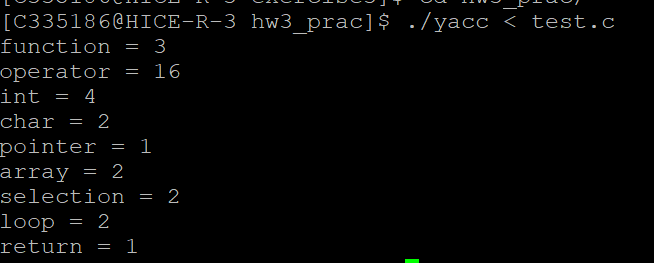
\includegraphics[width=1\linewidth]{스크린샷 2025-05-16 094737.png}
    \caption{Enter Caption}
    \label{fig:enter-label}
\end{figure}

이렇게 결과가 잘 출력된 것을 확인할 수 있다!

\end{document}

